\documentclass[../talk.tex]{subfiles}
\begin{document}

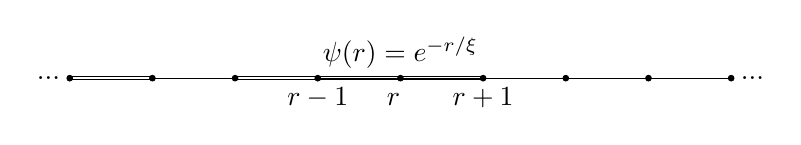
\begin{tikzpicture}[scale=.7]
    		\newcommand{\orig}{-1.5}
    		\newcommand{\trans}{1.5}
    		\newcommand{\vertspac}{-2.}
    	
    		% initial chain
    	
    		% bonds 
        	\draw[-,double] (\orig+\trans,0) -- (\orig+2*\trans,0) node [midway, above] {};
			\draw[-] (\orig+2*\trans,0) -- (\orig+3*\trans,0) node [midway, above] {};	
			\draw[-,double] (\orig+3*\trans,0) -- (\orig+4*\trans,0) node [midway, above] {};
			\draw[-,double] (\orig+4*\trans,0) -- (\orig+5*\trans,0) node [midway, above] {};
			\draw[-,double] (\orig+5*\trans,0) -- (\orig+6*\trans,0) node [midway, above] {};
			\draw[-] (\orig+6*\trans,0) -- (\orig+7*\trans,0) node [midway, above] {};
			\draw[-] (\orig+7*\trans,0) -- (\orig+8*\trans,0) node [midway, above] {};
			\draw[-] (\orig+8*\trans,0) -- (\orig+9*\trans,0) node [midway, above] {};
			
			% wavefunction
			\draw (\orig+4*\trans,0) -- (\orig+6*\trans,0) node [midway, above] {$\psi(r) = e^{- r/\xi}$};
    	
    		% sites
		    \filldraw (\orig+1*\trans,0) circle (0.05) node [left] {...};
		    \filldraw (\orig+2*\trans,0) circle (0.05) node [below] {};
		    \filldraw (\orig+3*\trans,0) circle (0.05) node [below] {};
		    \filldraw (\orig+4*\trans,0) circle (0.05) node [below] {$r-1$};
		    \filldraw (\orig+5*\trans,0) circle (0.05) node [below] {$r\phantom{1}$};
		    \filldraw (\orig+6*\trans,0) circle (0.05) node [below] {$r+1$};
		    \filldraw (\orig+7*\trans,0) circle (0.05) node [below] {};
		    \filldraw (\orig+8*\trans,0) circle (0.05) node [right] {};
		    \filldraw (\orig+9*\trans,0) circle (0.05) node [right] {...};
		      
		\end{tikzpicture}
\end{document}